\newpage
\chapter{Week 05: Implementation 4}
\section{Main work }

This week the works are mainly concentrated following points:


\begin{enumerate}
\item[*] Improvement in training technique-> wasserstein GAN with gradient penalty(WGAN-GP), TTUR(discriminator uses higher learning rate)
\item[*] Higher resolution -> use deeper network to generate higher resolution; test MSG-GAN
\item[*] Add condition to control the output 
\item[*] data augmentation, (random horizontal/vertical flip, random crop with random size and then resize )
\item[*] help features, e.g. checkpoint and recover from checkpoint, speed up(reduce for loop while loading data and some other calculation), more friendly argparse operation, summary the network(torchsummaryX)
\end{enumerate}
\paragraph{
	\\
 }


\section{WGAN-GP}
\paragraph{
the calculation of wgan-gp follows the famous paper of "Improved Training of Wasserstein GANs", the change in prior DCGAN is two points: remove the last layer sigmoid activate in discriminator, use the loss. The formula of new loss is as $D_w(\widetilde{x}) - D_W(x) + \lambda(\| \nabla_{\hat{x}} (D_w(\hat{x})))$ with $\hat{x}$ is created from $\hat{x}=\epsilon x + (1-\epsilon) \widetilde{x}, \epsilon \sim \mathbf{U} (0, 1) $. With the help of WGAN-GP, the training process is highly speeded up. We showed a example at figure \ref{fig:comparison}. We can see a significant improvement. Just in the 4th epoch, the DCGAN can learn to generate some figure, although it is still very blurry, while DCGAN still doesn't learn.
}

% \paragraph{
% our code is implemented as follows, significant improvment is at line 2, it calculate batch data's gradient effciently.
% }
Our code is implemented as follows, significant improvement is at line 2, it calculate batch data's gradient efficiently.


\begin{lstlisting}
    # gradient penalty
    grad_p_x = torch.autograd.grad(p_mix.sum(), data_mixed, retain_graph=True, create_graph=True)[0]
    # p_mix.sum(), trick to cal \par y_i / \parx_i independentl
    assert grad_p_x.shape == data_mixed.shape
    grad_norm = torch.sqrt(grad_p_x.square().sum(axis=(1, 2, 3)) + 1e-14)
    loss_2 = self.gp_lambda * torch.square(grad_norm - 1.)
\end{lstlisting}

\begin{figure}[htbp]
    \centering
    \subfigure[DCGAN at step4]{
    	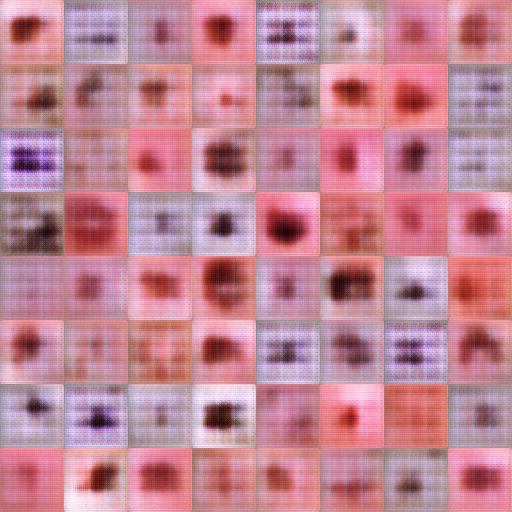
\includegraphics[width=2.1in]{images/week5/DCGAN_step4.png}
    }
 	\quad
    \subfigure[WGAN at step 4]{
    	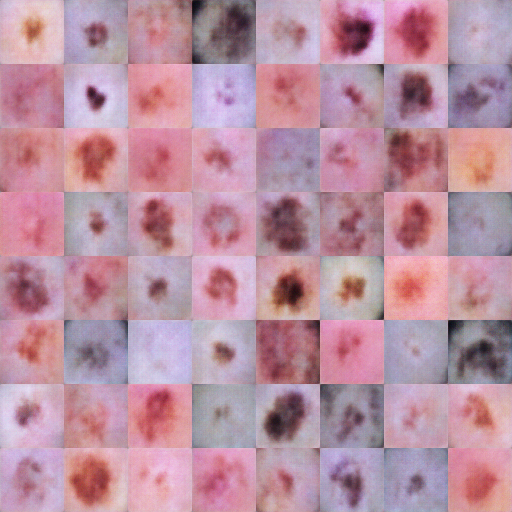
\includegraphics[width=2.1in]{images/week5/WGAN_step4.png}
    }\\
    \caption{Camparison of DCGAN and WGAN-GP}
    \label{fig:comparison}
\end{figure}
    

           
\section{Higher resolution}
\paragraph{
The standard DCGAN uses five layers and every layer uses 4*4 conv/convtrans kernel. We enlarge the depth to try generate the result,i.e. we add more layers in the hidden layer with 4*4 conv/conv\_trans to enlarge the depth. So we can control the generated figure's resolution. Depth 5 -> 64*64, Depth 6 -> 128*128, Depth 7 -> 256*256. And so on. We showed a result for 128x128 in figure \ref{fig:w_dc_gan_128}.
}

\paragraph{
In the training, 256*256 is still acceptable(90M params, 13.7G Mult-adds), but 512*512 is too huge for our training. Insteadly, we tried MSG-GAN, (Multi Scale Gradient GAN), which is a very interesting work. We use the author's code, (https://github.com/akanimax/BMSG-GAN). However, it requires too huge calculation resource and takes so long time. The result is still not very good. Although we tried in 4 RTX2080Ti with 100\% data, and 1 GTX1080 with 60\% data and trained for 2 days. But we think MSGGAN should work, since we tried a smaller MSGGAN network with depth 5 (generate from 4*4 to 64*64) for 179 epoch with roughly 30\% HAM10000 dataset, it learns something, although still very unclear. The results are showed in figure \ref{fig:msg_gan}
}
\begin{figure}[htbp]
    \centering
    \subfigure[W-DCGAN with GP, 128*128 resolution]{
    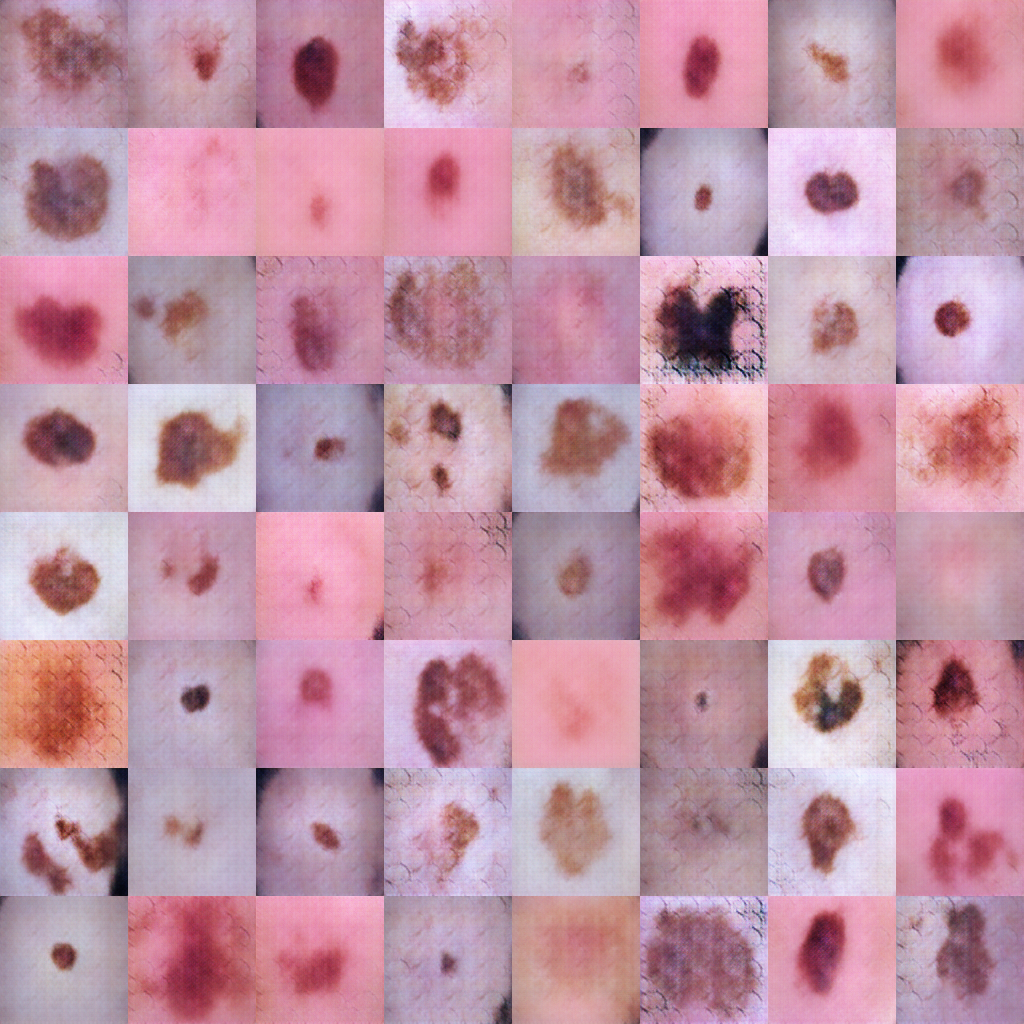
\includegraphics[width=2.1in]{images/week5/GAN 128_128.png}
    \label{fig:w_dc_gan_128}
    }
    \subfigure[MSG GAN for depth 5(max resolution 64*64)]{
    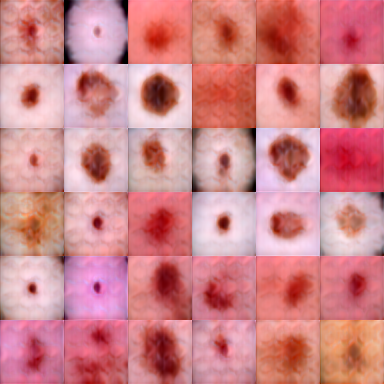
\includegraphics[width=2.1in]{images/week5/MSG_dep5_64_64.png}
    }
    \subfigure[MSG GAN for depth 7(max resolution 256*256)]{
    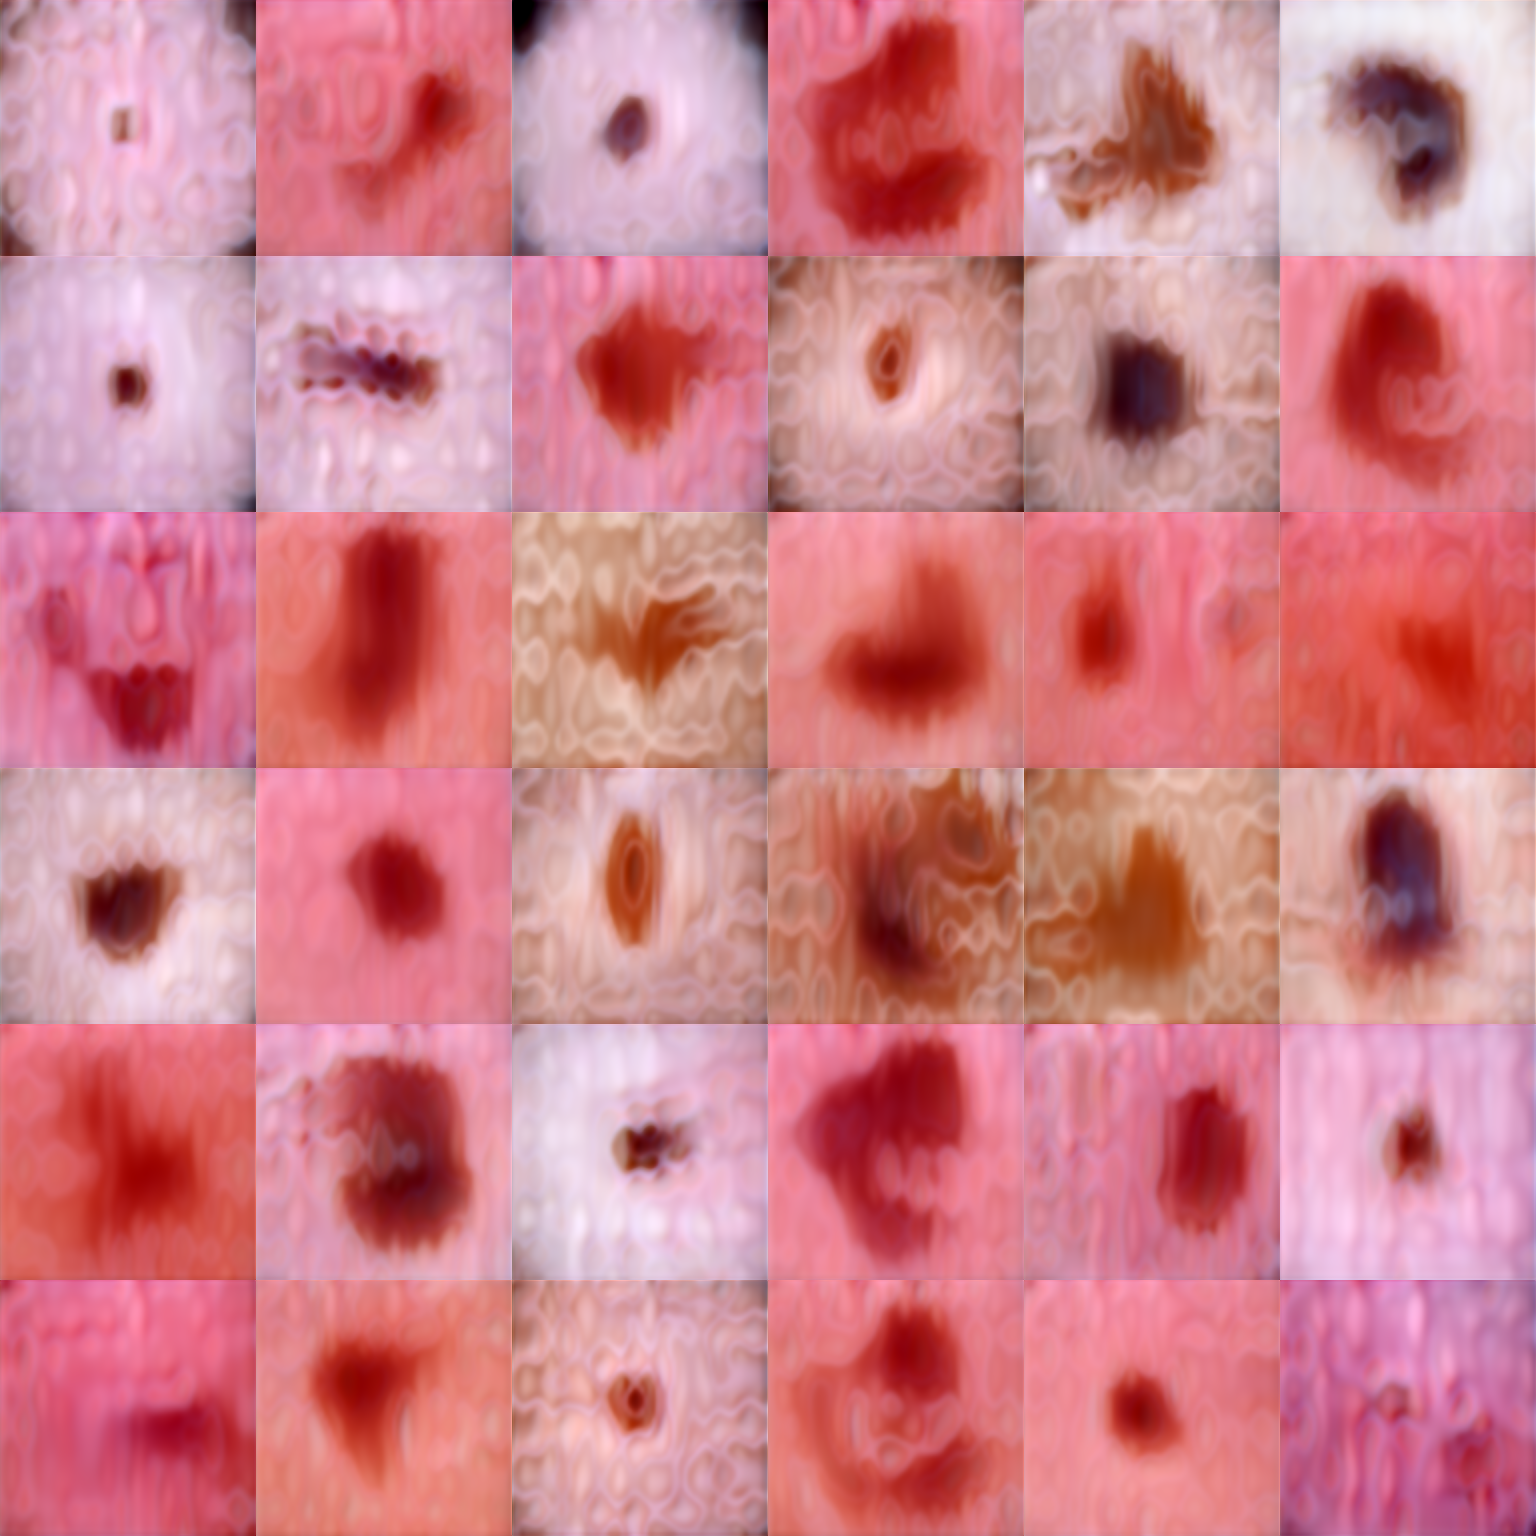
\includegraphics[width=2.1in]{images/week5/MSG_GAN7_256x256.png}
    }
    \caption{Some result of MSGAN}
    \label{fig:msg_gan}
\end{figure}

\section{condition}
\paragraph{
We add disease type as condition for training the network. }
\paragraph{
Firstly, add embedding layer in both generator and discriminator for label disease type. 
}
\paragraph{
Secondly, for generator, we concatenate the noise and embedded label as input. }
\paragraph{
Thirdly, for discriminator, originally the last layer should be conv-kernel with 4*4 size and 1 output channel so as to make sure that the output will be (batch\_ size, 1), 
we change the kernel as (n\_input\_channel, output\_channel=64, size=4*4). So the output would be (batch\_size, 64). Then similarly to generator, we concatenate the output and embedded label and feed into a new linear layer.}
\paragraph{ The result is shown in figure \ref{fig:cgan}. However, due to the time and calculation resource, we have not well trained the result. Every line is one class, although not well trained, we can see that truly  there is different style between different lines.}




\begin{figure}[htbp]
    \centering
    
    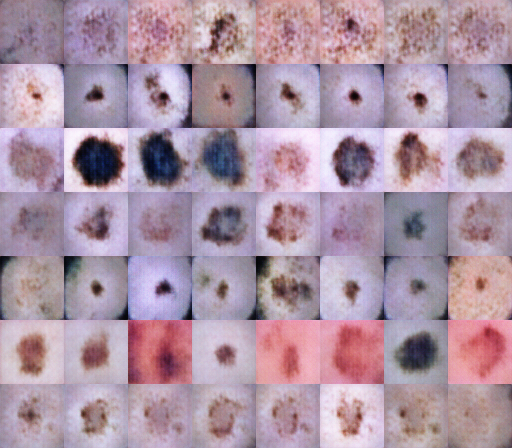
\includegraphics[width=2.1in]{images/week5/cGAN.png}
    
    \caption{conditional W-DCGAN with gp }
    \label{fig:cgan}
\end{figure}